\begin{frame}
\begin{figure}[htbp]
\begin{center}
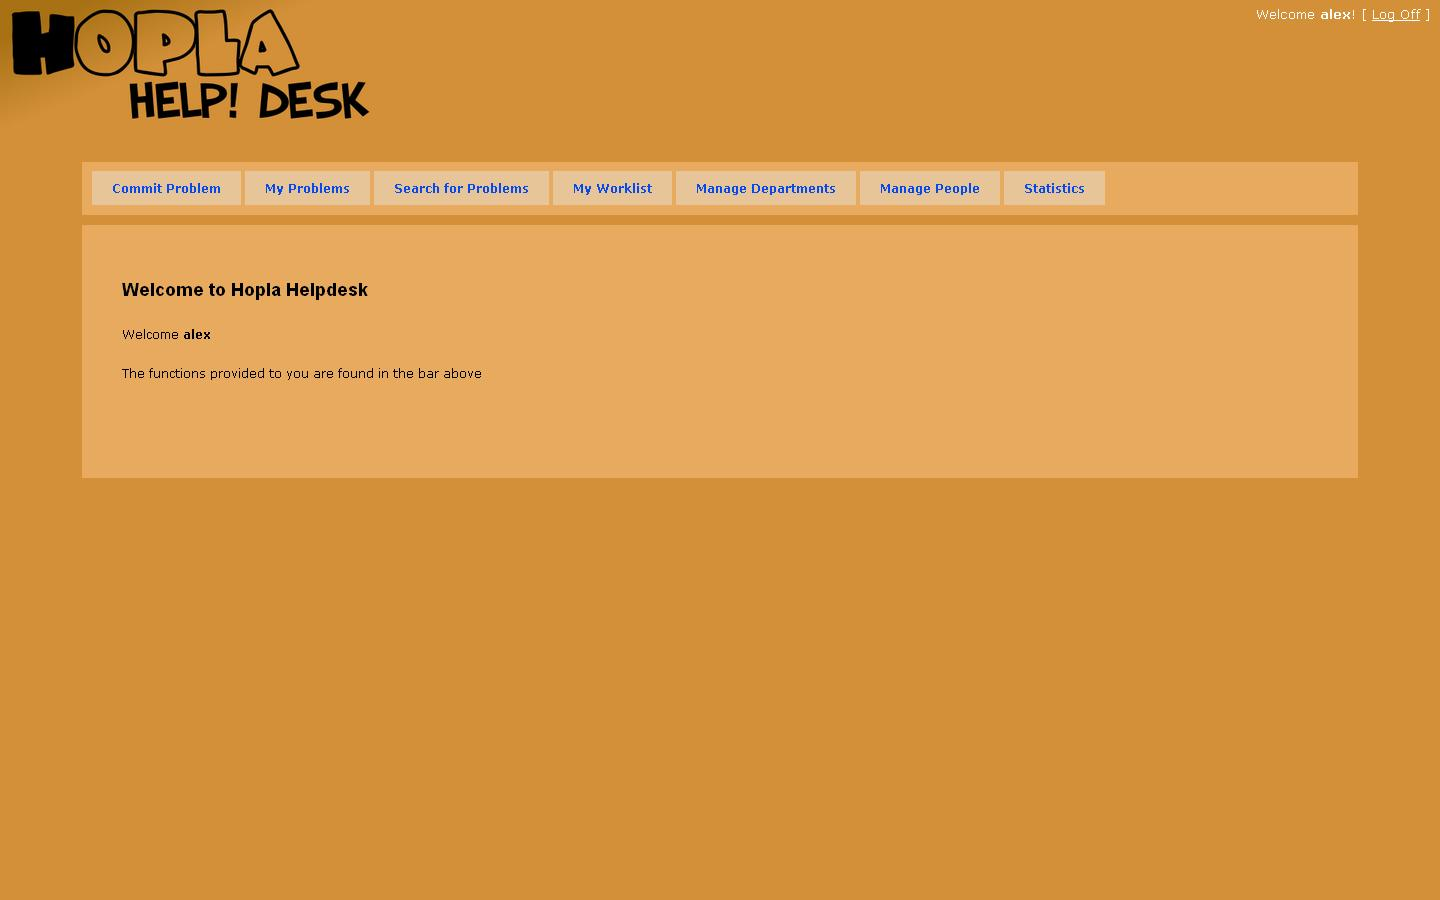
\includegraphics[]{input/search/home.JPG}
\caption{default}
\label{default}
\end{center}
\end{figure}

\end{frame}

\begin{frame}

\begin{figure}[htbp]
\begin{center}
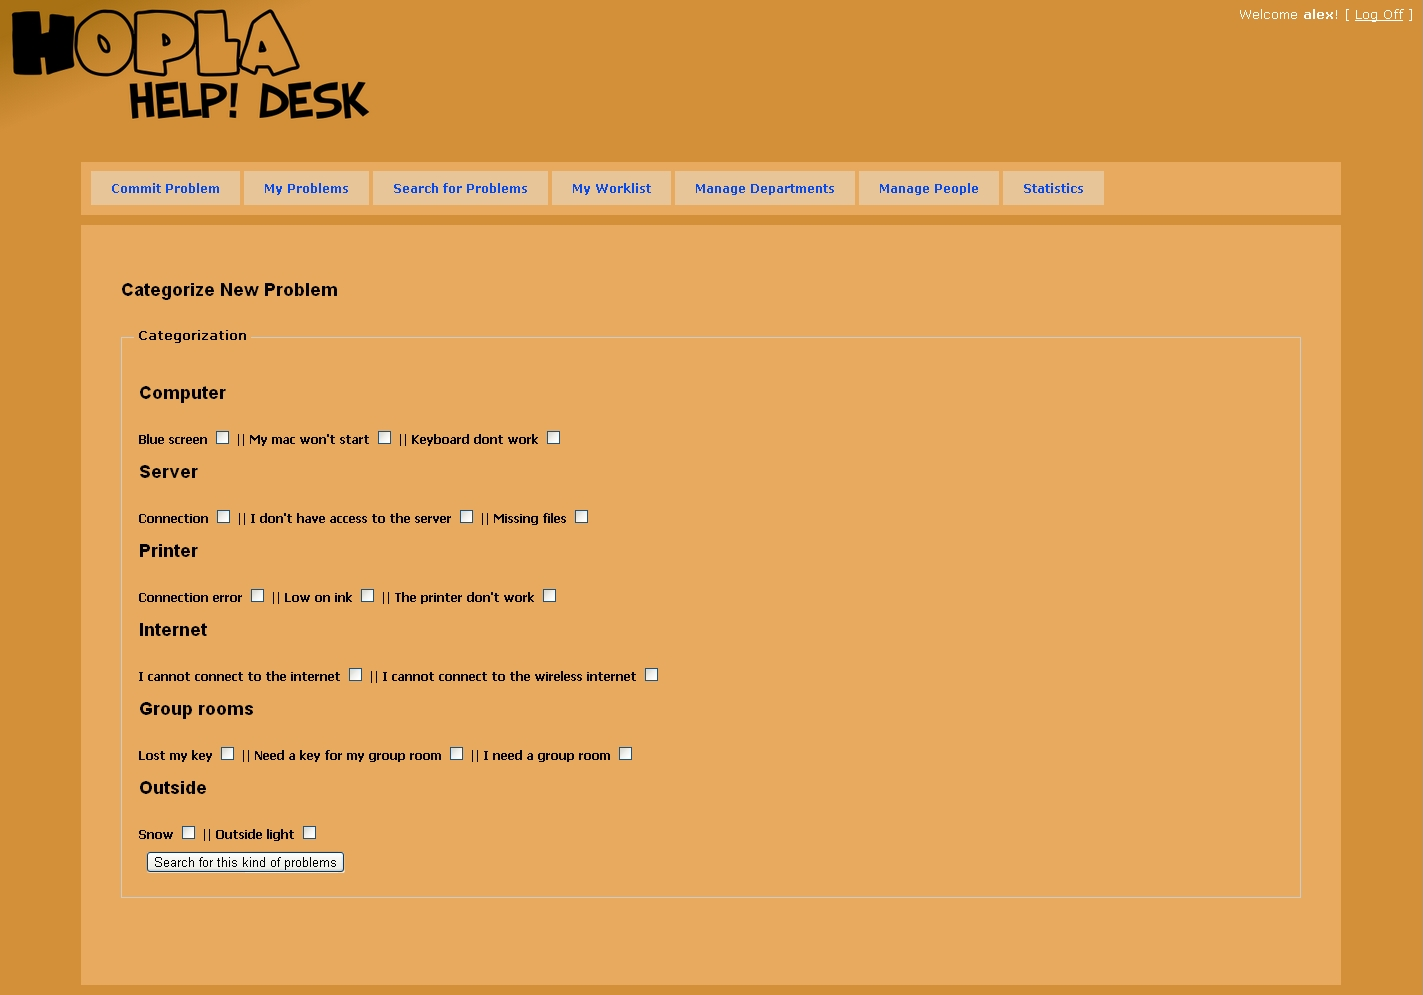
\includegraphics[]{input/search/commit.png}
\caption{default}
\label{default}
\end{center}
\end{figure}

\end{frame}

\begin{frame}

\begin{figure}[htbp]
\begin{center}
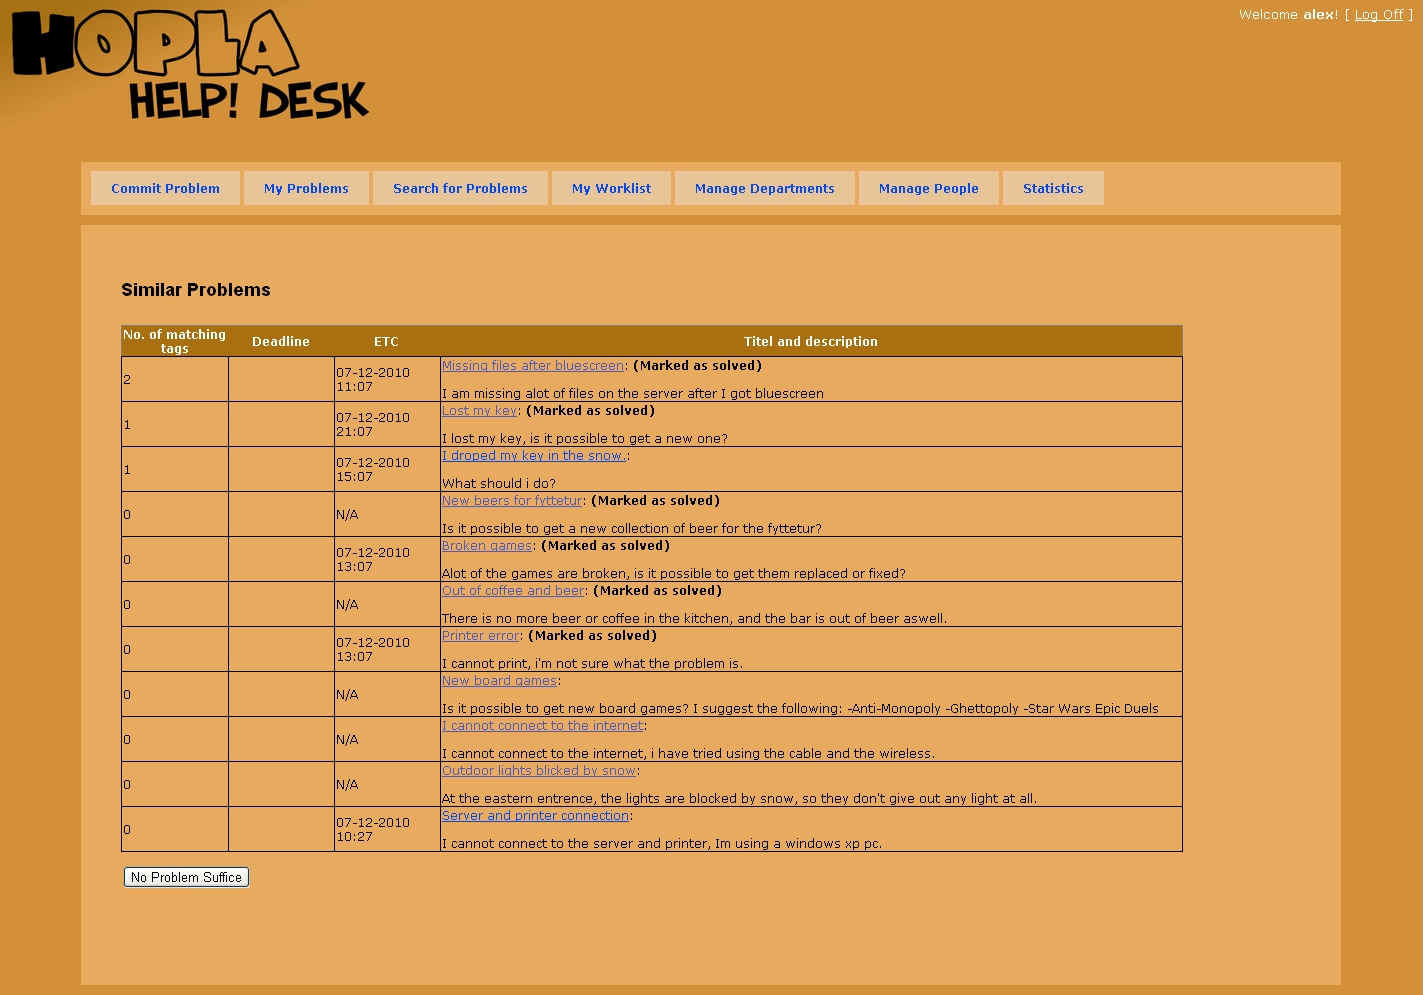
\includegraphics[]{input/search/similarProblems.png}
\caption{default}
\label{default}
\end{center}
\end{figure}

\end{frame}

\begin{frame}

\begin{figure}[htbp]
\begin{center}
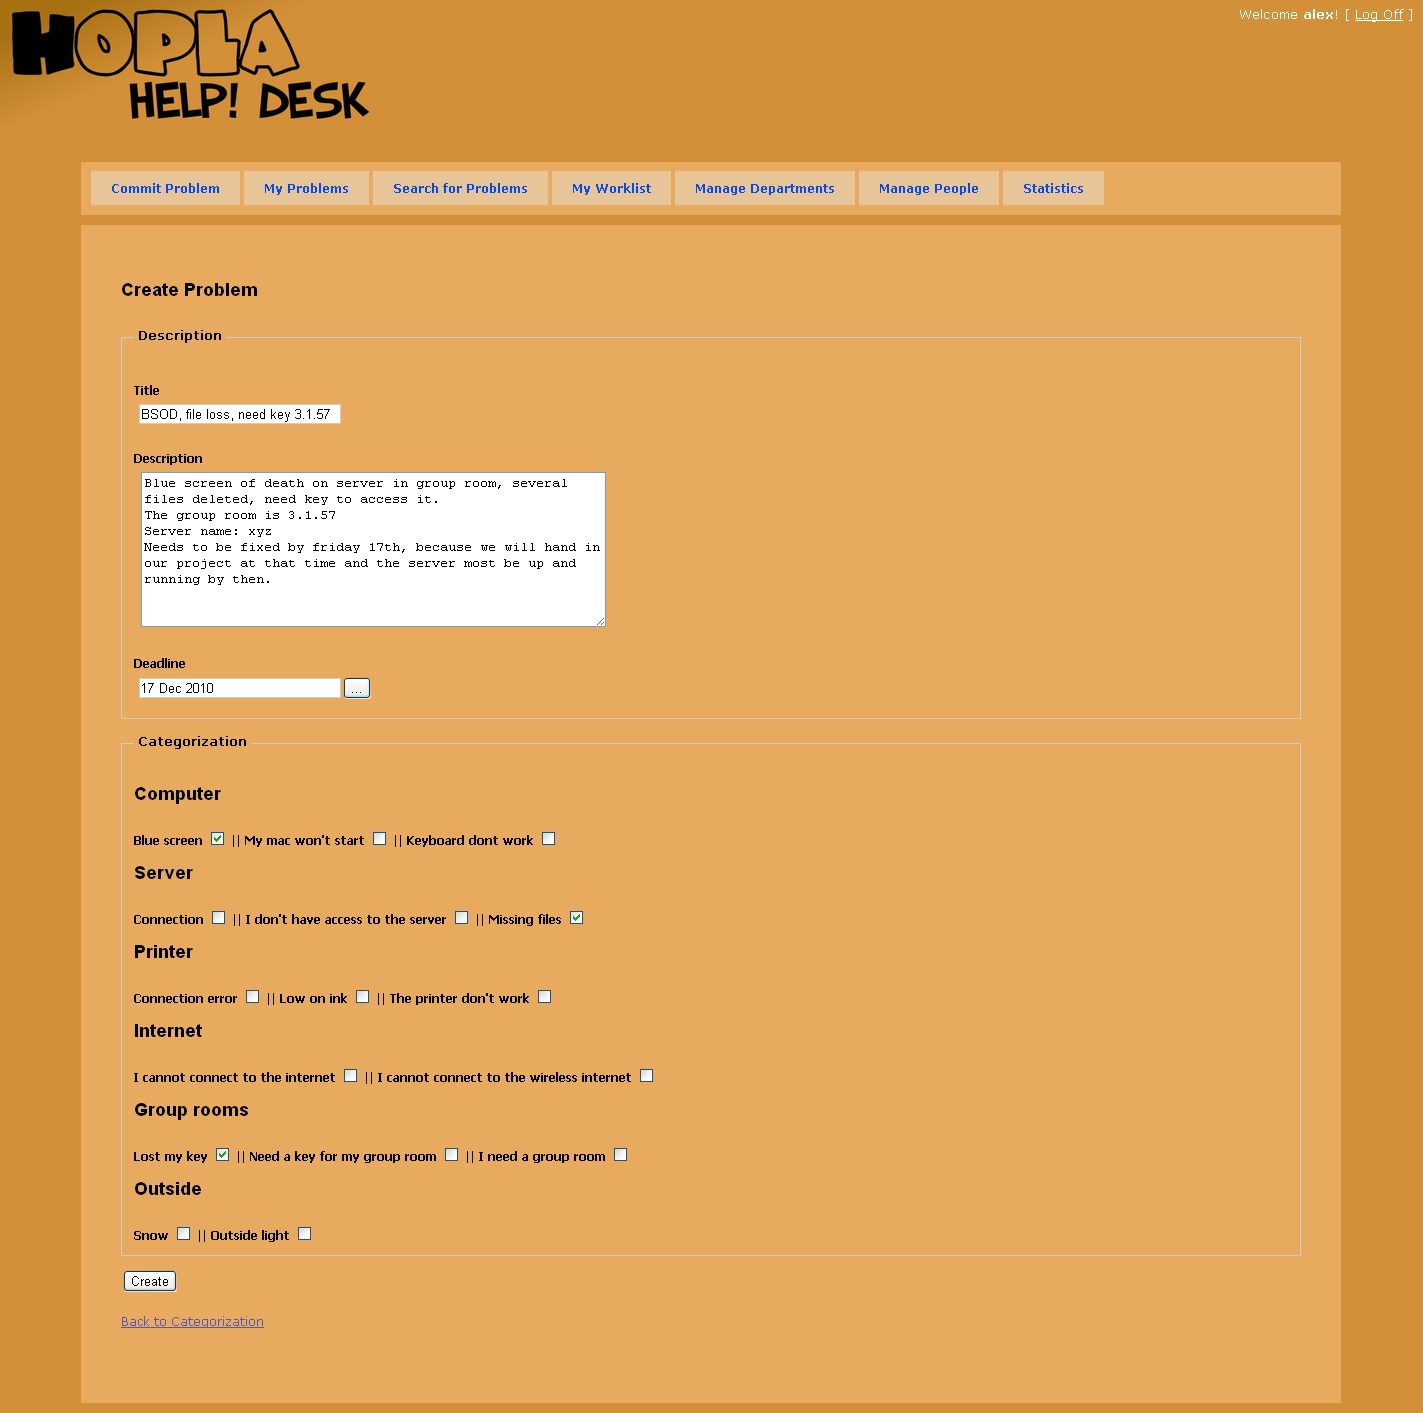
\includegraphics[]{input/search/newProblem.png}
\caption{default}
\label{default}
\end{center}
\end{figure}

\end{frame}
% The interresting here is the search, we try search a set of problems

\begin{frame}{The Search}
\begin{itemize}
\item Tags to search: Computer + Bluescreen
\item Minimum number of problems to find: 3
\end{itemize}

\end{frame}



\begin{frame}{The Search}
\begin{itemize}
\item Tags to search: Computer + Bluescreen
\item Minimum number of problems to find: 3
\end{itemize}

\end{frame}

